\chapter{Introducción}

\section{Seguridad de los dispositivos informáticos}

En un contexto marcado por el explosivo crecimiento de las tecnologías de la información, la vida de las personas se encuentra ligada al uso de dispositivos electrónicos, y expuesta a las vulnerabilidades que éstos presentan.

La aparición del comercio virtual y la banca electrónica, los dispositivos del internet de las cosas (\acrshort{iot}), la nube y los teléfonos inteligentes, entre otros, dan lugar a un escenario dónde, cada vez más, aquellos dispuestos a explotar las vulnerabilidades de los sistemas pueden lucrarse y perjudicar gravemente si no se toman las medidas para evitarlo. 

Pérdidas de datos, robo o bloqueo de información, suplantaciones de identidad, e incluso la posibilidad de infectar los computadores con software que permita al atacante utilizarlos para su propio beneficio (ataques DDoS o minado de bitcoin, por ejemplo), son algunas de las amenazas a las que se está expuesto hoy en día en Internet.

En este marco surgen constantemente herramientas para asegurar la protección los dispositivos, tanto de los datos sensibles como de la disponibilidad de los mismos, ya sea porque un ataque inhabilite un servicio o cierto tipo de \Gls{Malware} impida acceder a los dispositivo de forma regular (\gls{Ransomware}) \cite{independiente, cnncert}. 

\begin{figure}[hbtp]
  \centering
  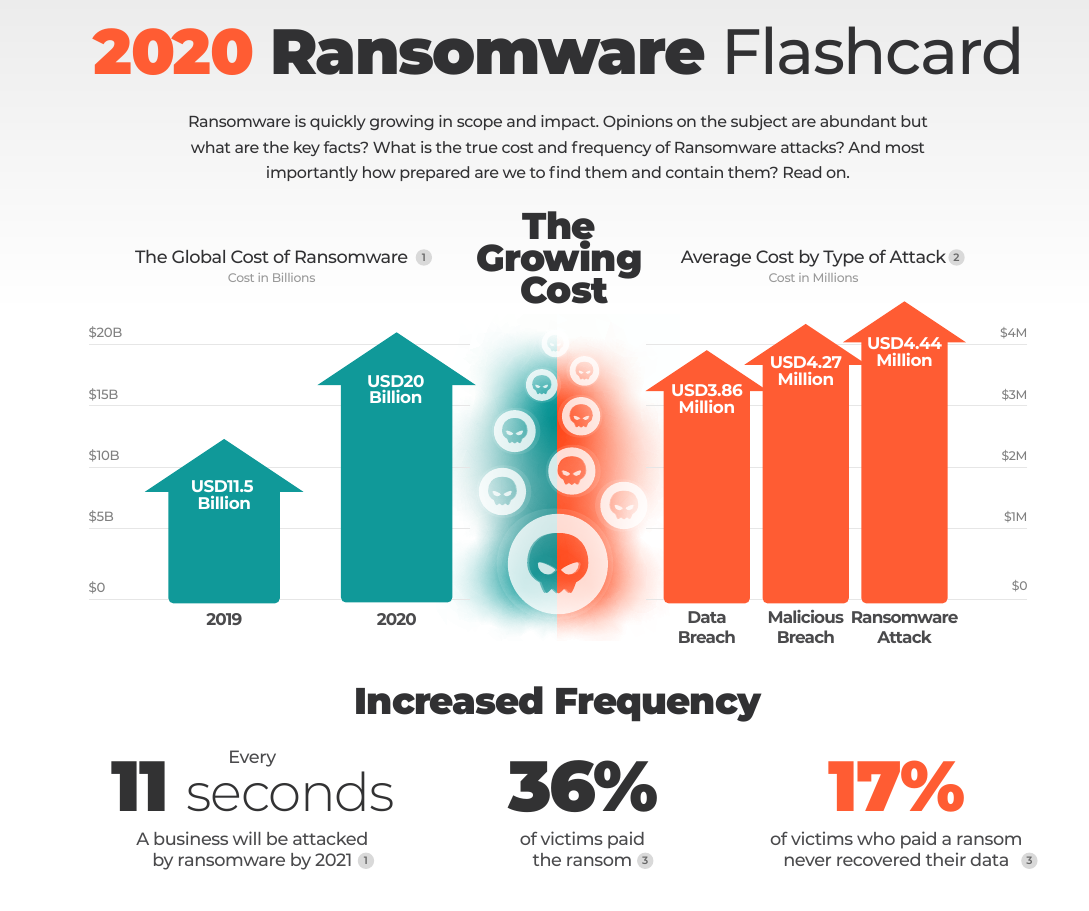
\includegraphics[width=0.8\textwidth]{imagenes/ransomware1.png}
  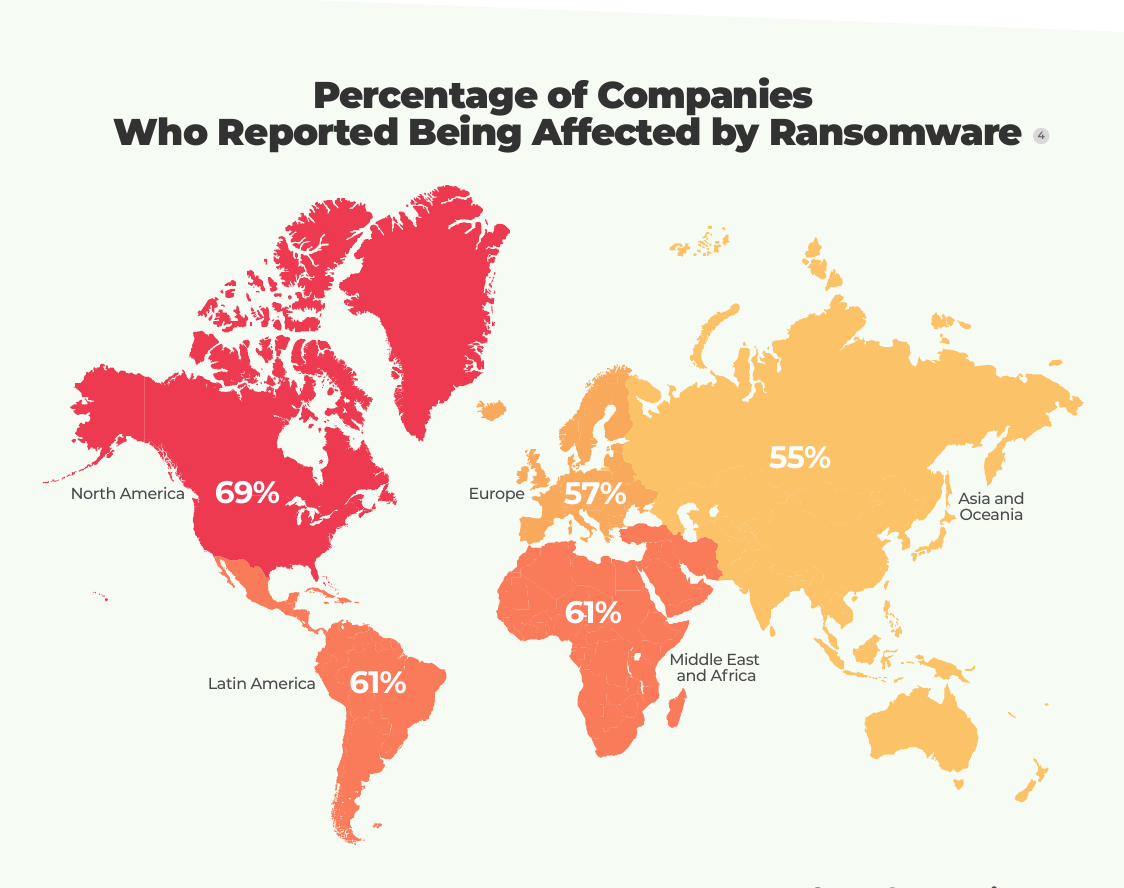
\includegraphics[width=0.8\textwidth]{imagenes/ransomware2.png}  
  \caption{Gráficos extraídos del informe citado del CNN en el que se muestran algunas tendencias de las incidencias relacionadas con \gls{Ransomware} \cite{cnncert}}
\end{figure}


Entre todas estas herramientas aparece \textbf{\textit{Wazuh}}\footnote{Ver \url{https://wazuh.com/}\cite{WAZUH}}, una plataforma \gls{OpenSource} de ciberseguridad que pretende convertirse en un estándar y una referencia a la hora de proteger los dispositivos informáticos y que engloba distintos tipos de módulos o herramientas que ofrecen, entre otras cosas, recolección y análisis de los registros (\textit{logs}) de los \textit{endpoints} \footnote{Un endpoint es cualquier dispositivo remoto conectado a una red y que genera tráfico de datos: un ordenador portátil, una teléfono móvil, un servidor o incluso un dispositivo IOT}, detección de vulnerabilidades en el software instalado, control de la integridad de archivos sensibles o detección de intrusiones (HIDS).


Wazuh es una herramienta que permite recopilar y analizar información sobre eventos de ciberseguridad que tienen lugar en los sistemas de una organización y alertar a sus responsables cuando dichos eventos tengan una importancia determinada. Sin embargo, esta monitorización requiere de una configuración y puesta a punto previa y no siempre se cumplen los requisitos para \textbf{analizar todas las posibles amenazas}. Si no se trata de sobrepasar las defensas de un sistema, difícilmente se puede saber cómo de seguras son estas. Esta es la razón por la que existen los llamados \textbf{Hackers éticos} y sus \textbf{test de penetración de sistemas}, de los que hablaremos a continuación. En este proyecto se va a analizar el uso de Wazuh (se analizará más adelante su estructura y funcionamiento) y la relación que tienen (o que pueden tener) este software y el \textbf{Hacking ético}.

\begin{figure}[hbtp]
  \centering
  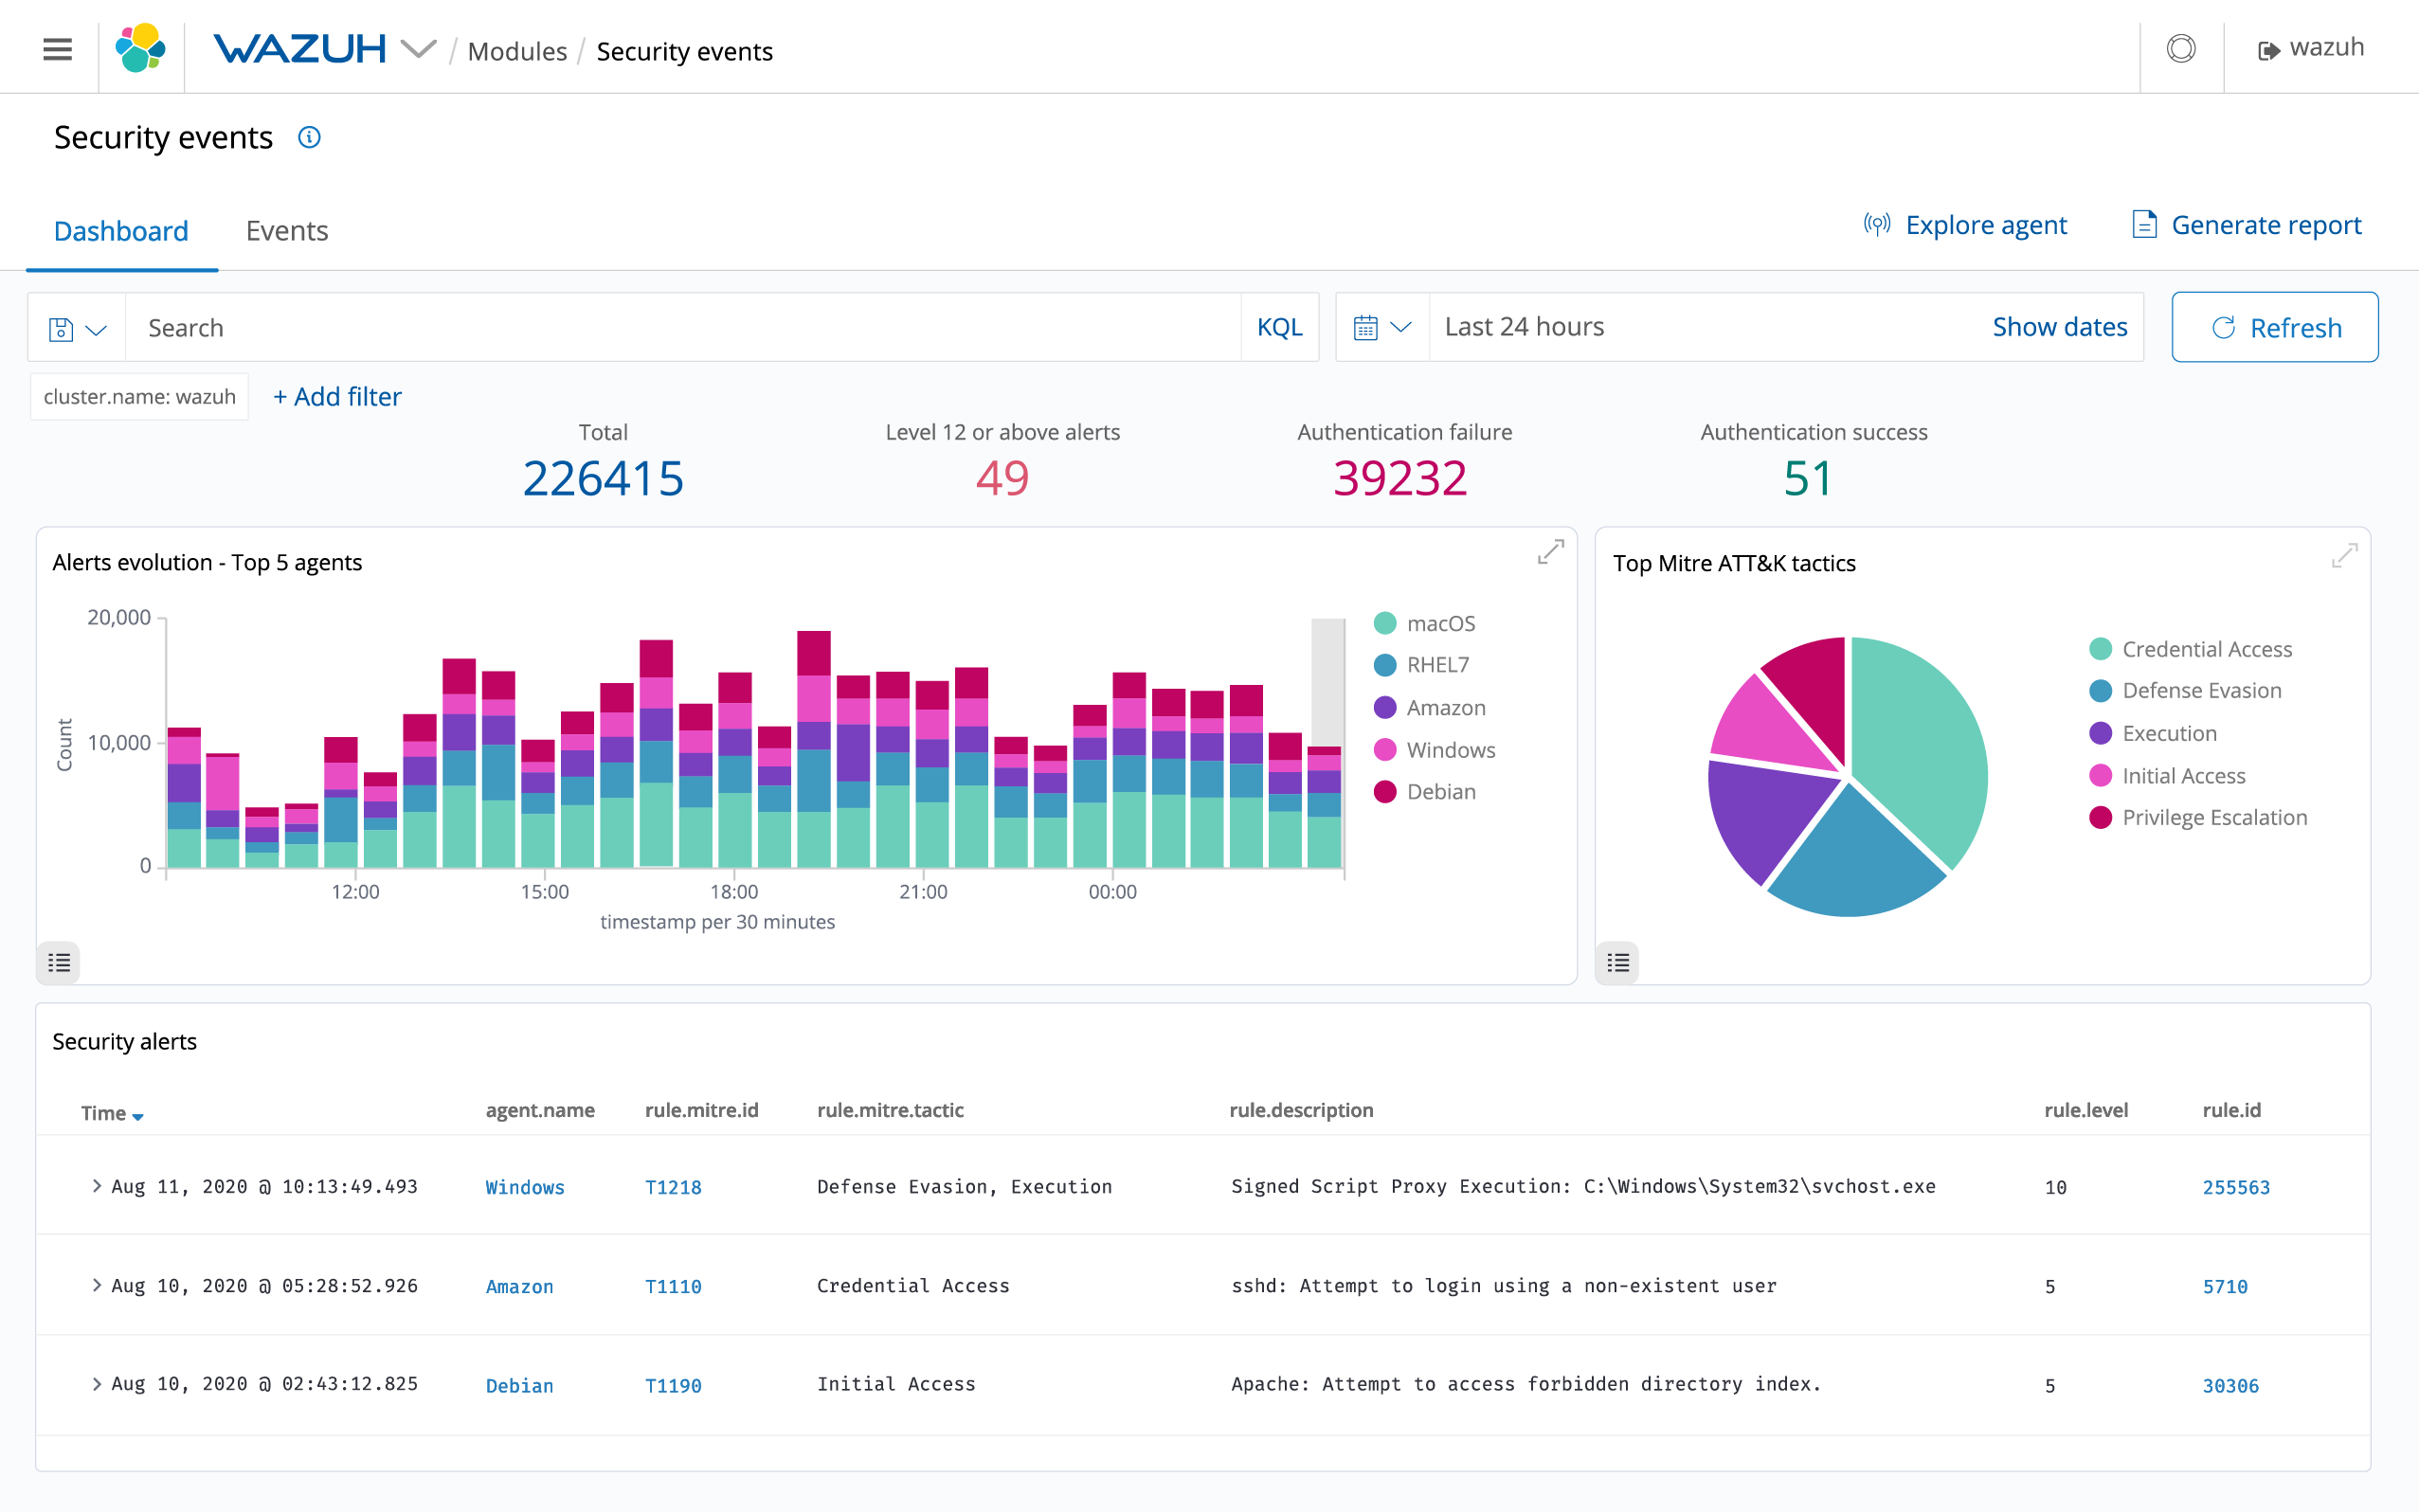
\includegraphics[width=0.8\textwidth]{imagenes/wazuh_kibana.png}
  \caption{Ejemplo de visualización de la interfaz web de Wazuh en la pestaña de `eventos de seguridad'. En ella se aprecian algunas estadísticas de alertas generadas en los sistemas monitorizados.}
\end{figure}

\subsection{\textit{Hacking} ético y seguridad ofensiva}

Un hacker ético es una persona con conocimientos técnicos suficientes que emplea sus habilidades en un marco legal y con fines éticos. Normalmente, son contratados por empresas y cuentan con permiso explícito de la misma para tratar de ganar acceso de forma `ilícita' a los sistemas y a la información de la misma, poniendo a prueba la seguridad de su entorno y realizando un informe o reporte con las conclusiones extraídas. Existen principalmente dos roles que se enmarcan dentro del hacking ético, los analistas que realizan `tests de penetración de sistemas' y aquellos que participan en los programas de \gls{bugb}.

Hoy en día existen multitud de organizaciones en el ámbito de la ciberseguridad que desarrollan herramientas y comparten recursos para los denominados test de penetración de sistemas, en los que buscan extraer toda la información posible de un servidor por medio de técnicas como el escaneo de puertos, descifrado de contraseñas, análisis de redes (\gls{network sniffing}) o \gls{Reverse engineering}. 

Entre ellas cabría destacar la organización \textbf{Offensive security}\footnote{https://www.offensive-security.com/ \cite{offensive}} que ofrece formación y certificaciones para hackers éticos y es muy conocida por ser la creadora de proyectos como \textbf{Kali Linux}\cite{kalilinux}, una distribución de Linux orientada a tests de penetración de sistemas (como \textbf{Black Arch Linux} o \textbf{Parrot OS}) con diferentes configuraciones y herramientas\cite{tools} por defecto dirigidas a facilitar las tareas de un auditor y por sus certificaciones relacionadas con ciberseguridad, que son altamente apreciadas por la comunidad.

\section{Motivación}

Wazuh engloba diversos módulos y herramientas que se enmarcan dentro de las labores de un analista de ciberseguridad y que permiten detectar amenazas cuando estas ocurran y defender los dispositivos de posibles ataques, así como detectar las intrusiones como parte de un análisis forense (\gls{forensics}).

Es un software \textbf{libre y gratuito (\acrshort{FOSS})} y parte del éxito de la empresa se debe a su fuerte comunidad (Open-Source) y a que se trata de un proyecto moldeable y que se adapta a las cambiantes necesidades del entorno de la ciberseguridad actual. 

Sin embargo, hoy en día son fundamentales para los departamentos de seguridad de las empresas las auditorías de seguridad (o tests de penetración de sistemas) y las búsquedas de errores por cuenta ajena (comúnmente conocidas como \gls{bugb}) en las que se trata de poner a prueba un entorno \textbf{desde un punto de vista externo al mismo}, pudiendo encontrarse a veces vulnerabilidades que escapan al alcance de herramientas como Wazuh.

Además, dado que Wazuh es uno de los elementos que utilizan muchas empresas para defenderse de ataques, es también un \textbf{factor más a analizar durante las auditorías de ciberseguridad} o tests de penetración de sistemas. 

Es por ello que se plantean dos ideas importantes sobre la \textbf{relación entre Wazuh y el hacking ético}.

\begin{itemize}
    \item ¿Qué pueden aportar los tests de penetración o las técnicas de \gls{bugb} a la seguridad de un sistema que ya cuenta con Wazuh?
    \item ¿Que puede aportar Wazuh a aquellos que practican el Hacking ético?
\end{itemize}

\subsection{Relación entre Wazuh y el Hacking ético}

Durante este trabajo se tratará de analizar esta relación entre un software `defensivo' y técnicas `ofensivas' que se utilizan como un adversario para evaluar y conseguir mejorar las medidas defensivas de los entornos. 

Por un lado, un test de penetración de sistemas puede sacar a la luz \textbf{vulnerabilidades o defectos}\cite{owasp} del sistema que \textbf{quizá hayan pasado por alto a los mecanismos del software defensivo} (puesto que un software defensivo no siempre puede detectar todos los eventos de seguridad que ocurren en el sistema). De esta forma, el test serviría también para \textbf{evaluar el rendimiento} de la herramienta defensiva (Wazuh, para el caso que nos ocupa) y \textbf{detectar posibles mejoras para el mismo}, ya sea por medio de nuevos módulos o mejorar en los existentes, o porque una escasa configuración de la herramienta la haya hecho ineficiente en un caso concreto y se requieran cambios en la misma.

Por otro lado, \textbf{Wazuh puede responder a una necesidad importante en el ámbito del hacking ético}, en el que la \textbf{recopilación y el almacenamiento} de la información extraída de los dispositivos analizados muchas veces se realiza en ficheros de texto plano y sin un formato específico, lo que \textbf{hace difícil su análisis y distribución}. Wazuh cuenta con bases de datos internas y un motor de alertas que se integra con Elasticsearch, y tiene su propia interfaz web con visualizaciones de datos y varios motores de análisis de información de seguridad. Si se pudiera enviar la información de los test de penetración (o similares) a Wazuh para que fuera analizada, decodificada e indexada en un motor de búsqueda como es Elasticsearch, \textbf{se estaría supliendo una de las necesidades más básicas de cualquier hacker ético}. Además, dentro de la comunidad de hacking ético se anima a \textbf{tratar de automatizar todos los procesos que se pueda}, especialmente la recopilación y análisis inicial de información de los sistemas (por ejemplo en la charla que citamos de \cite{hakluke}\footnote{Ver \cite{hakluke}, How to Crush Bug Bounties in the first 12 Months} que habla sobre cómo prosperar en el mundo del Bug Bounty), y Wazuh podría ser un elemento clave para construir herramientas que permitan llevar esto a cabo.

Es por esto que consideramos muy importante comenzar a crear y/o mejorar la interacción entre el mundo del hacking ético y la comunidad de herramientas `defensivas' como Wazuh. 

\subsection{Oportunidad de negocio}

Además, dado que Wazuh es completamente gratuito. Los ingresos de la compañía no dependen de `ventas' de licencias o similares sino de otros \textbf{servicios como el soporte técnico o la \gls{cloud}} \cite{wcloud} de Wazuh. 

Dado que Wazuh es una herramienta altamente configurable, una mala (o insuficiente) configuración del software o la escasa formación de sus usuarios puede causar que queden partes del sistema, que podrían ser analizadas, sin monitorizar, o que eventos que Wazuh ha sido capaz de detectar no sean atendidos o no se tomen las medidas requeridas a tiempo.

Un aspecto interesante por tanto a valorar es la \textbf{oportunidad de negocio} que supondría integrar tests de penetración de sistemas junto con los servicios de soporte técnico que fueran \textbf{especializados} en comprobar y confirmar que Wazuh está correctamente configurado para analizar todos los puntos de interés de los distintos dispositivos de la empresa, así como de confirmar que los empleados y encargados de mantener los sistemas seguros sepan hacer un buen uso del software.  

De esta forma, utilizando conocimientos sobre hacking ético, cualquiera con conocimientos sobre el software de Wazuh podría ofrecer un servicio específico de auditoría de sistemas que incluya un test de penetración junto con la instalación o configuración de Wazuh. Analizando qué puntos está cubriendo el software y cuales podría cubrir con la configuración adecuada o por medio de mejoras en el mismo.

Para la compañía detrás de Wazuh, esta sería una oportunidad de generar \textbf{valor añadido} a sus ya existentes servicios (como el de soporte técnico) o incluso añadir nuevos servicios, basados en la seguridad ofensiva, para \textbf{afianzar clientes} o conseguir otros nuevos.

\section{Justificación y objetivos}

El objetivo de este trabajo es, por tanto, analizar la relación entre un software defensivo como Wazuh con aquellas técnicas y herramientas propias del hacking ético. Responder a las preguntas planteadas:

\begin{itemize}
    \item ¿Qué pueden aportar las técnicas de hacking ético a Wazuh?
    \item ¿Qué puede aporta Wazuh a los hackers éticos?
    \item ¿Cómo pueden relacionarse estos sistemas entre sí?
\end{itemize}

En primer lugar, y dado que consideramos que herramientas más complejas (como es el caso de Burp Suite, ver \cite{burp}) tienen su propio mecanismo de registros que pueden ser enviados a Wazuh y analizados con cierta facilidad, se propondrán y estudiarán distintos medios para \textbf{registrar los resultados de la ejecución de herramientas en consola de comandos} (como, por ejemplo, nmap, aircrack o Nikto), se evaluará la viabilidad de cada método y la posibilidad de integrarlos con Wazuh para indexar la información generada por estos.

Una vez hecho esto, se evaluará el rendimiento de Wazuh en un escenario que simule la realidad, instalándolo en una máquina vulnerable y sometiendo a esta a un test de penetración. La idea es detectar cómo puede Wazuh servir para detectar cierto tipo de ataques y cómo se podría mejorar la herramienta. De esta forma, se valorará la utilidad de emplear las técnicas de penetración de sistemas \textbf{para evaluar el rendimiento de Wazuh como herramienta defensiva}.

Por otro lado, evaluaremos qué se puede detectar (generar alertas o notificaciones ante eventos de importancia) usando el módulo desarrollado. Se estudiará cómo puede esto \textbf{complementar a la labor defensiva de Wazuh} y la correlación existente entre los eventos detectados por Wazuh (con sus módulos por defecto) y aquellos detectados usando la herramienta desarrollada. Es decir, revisaremos si la herramienta complementa a Wazuh, notificando de eventos que este pasa por alto o si sirve más bien para verificar desde otra perspectiva que Wazuh esté detectando los eventos correctamente.

En resumen, los objetivos principales del proyecto son:

\begin{itemize}
    \item Crear una herramienta que sirva de nexo entre Wazuh y las herramientas típicas de pentesting.
    \item Evaluar el aporte de las técnicas de hacking ético a la herramienta de Wazuh.
    \item Estudiar el valor que ofrece Wazuh a los hacker éticos en sus actividades.
\end{itemize}


\section{Estado del arte}\label{sec:estado del arte}

Existen diversas herramientas para el registro de eventos en los diferentes sistemas operativos, sin embargo, a día de hoy, no hay variedad en cuanto a herramientas que estén especializadas en recopilar o analizar los registros o las salidas generadas por herramientas propias de una auditoría de ciberseguridad y, en general, las opciones que existen están limitadas por uno u otro lado.

Las distintas soluciones y herramientas que existen para monitorizar o registrar la ejecución de comandos en una consola serán descritas posteriormente en el \autoref{cap:Registro}, si bien no ahondaremos más en ellas en esta sección sí que mencionaremos una herramienta existente cuyo propósito es bastante similar al que se define en este proyecto.

\subsection{Faraday: un entorno colaborativo de penetración de sistemas y administración de vulnerabilidades}

\begin{figure}[!hbt]
  \centering
  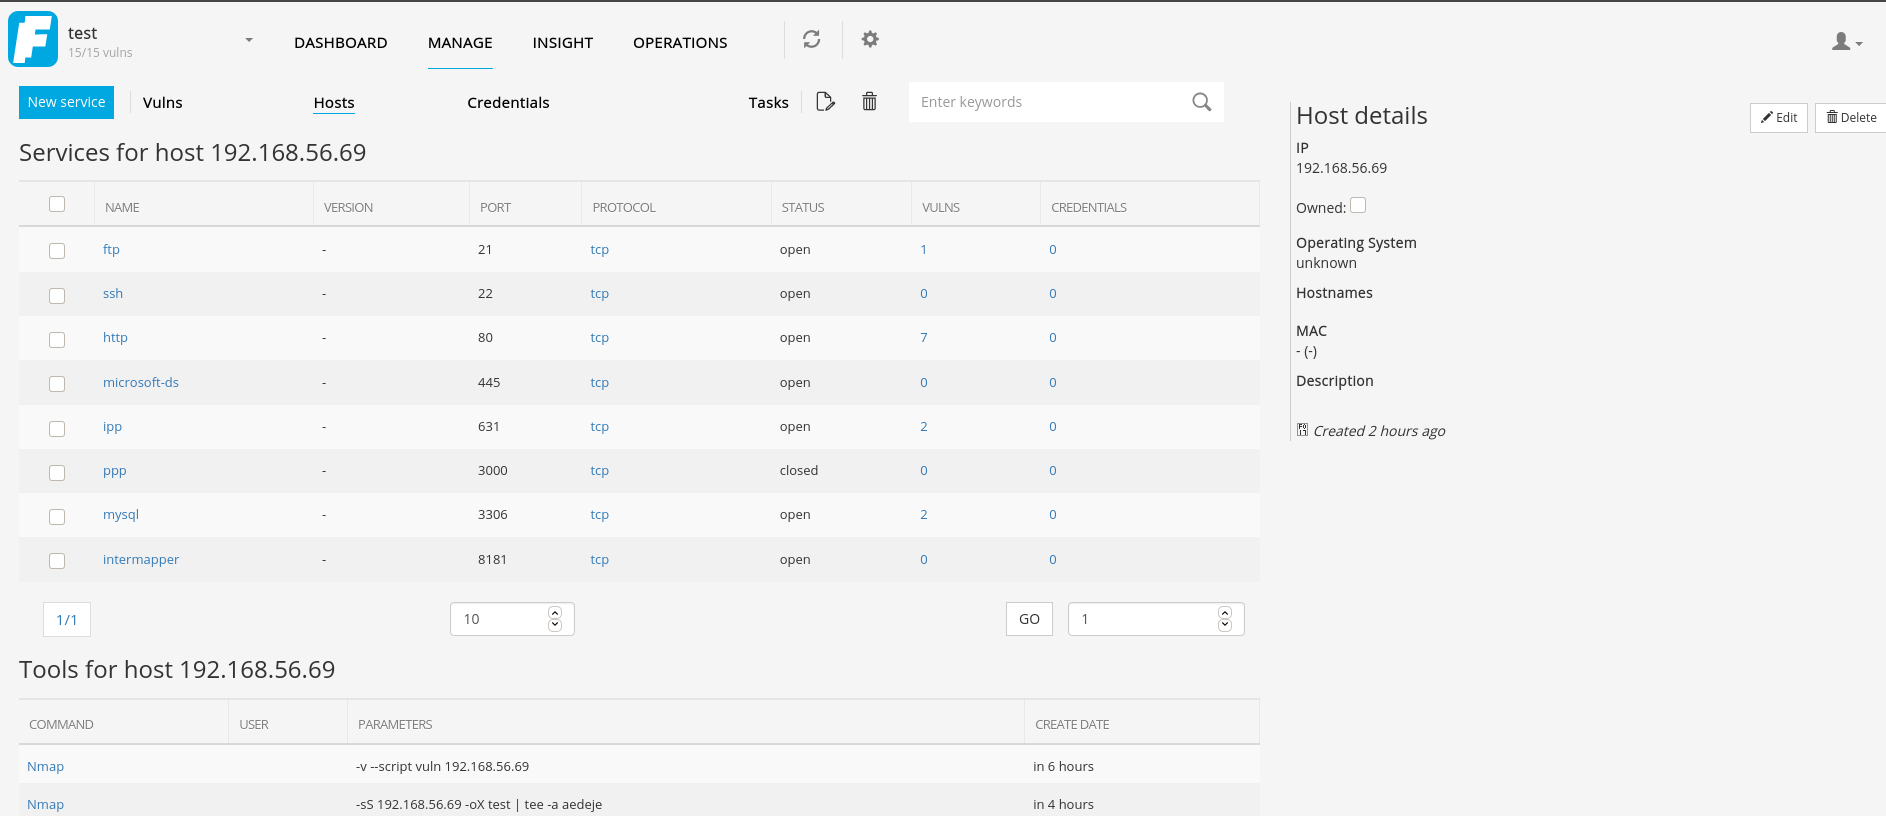
\includegraphics[width=\textwidth]{imagenes/faraday_host.png}
  \caption{Ejemplo de la ventana de hosts con la información extraída por Faraday usando nmap. Fuente: elaboración propia.}
  \label{faraday1}
\end{figure}

\begin{figure}[!hbt]
  \centering
  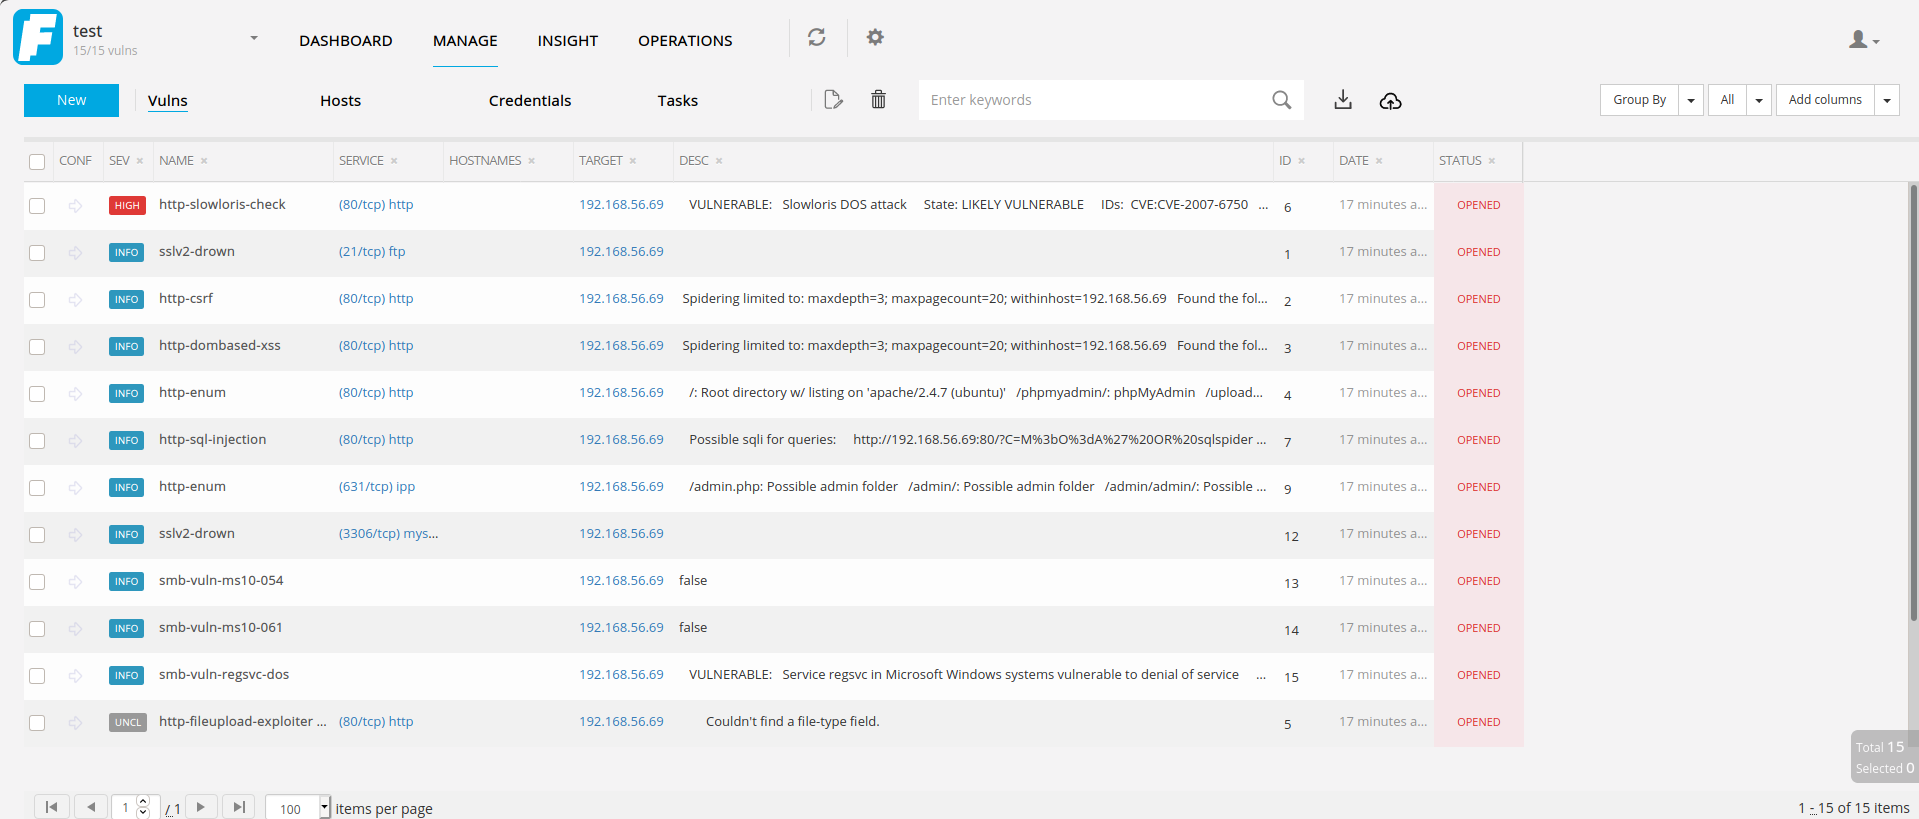
\includegraphics[width=\textwidth]{imagenes/faraday_vuln.png}
  \caption{Ejemplo de la ventana de vulnerabilidades de Faraday. Podemos visualizar las vulnerabilidades localizadas hasta el momento, su importancia. Fuente: elaboración propia.}
  \label{faraday2}
\end{figure}

\textbf{Faraday}\footnote{Ver \url{https://github.com/infobyte/faraday}} es un proyecto que pretende ofrecer una experiencia multiusuario de entorno de desarrollo para test de penetración de sistemas. Está diseñado para analizar datos extraídos de distintas herramientas de ciberseguridad e indexar los resultados del análisis de forma que tengan un formato analizable y fácil de compartir.

\subsubsection{Análisis de Faraday}

Faraday es un producto bastante nuevo, su primera \textit{release} disponible en Github data de finales de 2019 y tiene un soporte bastante activo en la actualidad. De hecho, es una de las herramientas que vienen por defecto en la distribución de Linux destinada a pentesting: Kali Linux.

Dispone de un servidor principal y varios clientes que se le conectan. El servidor utiliza un backend con una base de datos relacional postgreSQL. 

\begin{figure}
\begin{lstlisting}[language=bash,caption={Ejemplos de transformaciones de código hechas por Faraday}]
[1] sudo nmap -sS 192.168.56.69
[1] sudo nmap -oX /tmp/Nmap_04cgvggq.xml -sS 192.168.56.69 2>&1 | tee -a tmp.MCqWwd589v0Lk6l0bThFlEsrXWkhQ 

[2] sudo nmap -sS -oX test 192.168.56.69  | tee -a test_2
[2] sudo nmap -sS 192.168.56.69 -oX /tmp/Nmap_tuuvu2vm.xml | tee -a aedeje 2>&1 | tee -a tmp.qulP2E4IPQVgGzteTTQilsSOoe74c
\end{lstlisting}
\caption{Ejemplo de cómo transforma Faraday los comandos introducidos.}
\label{farday_transformation}
\end{figure}


Un primer detalle que llama la atención de su cliente es que dispone de una consola propia de comandos, integrada en una aplicación de escritorio y que modifica los comandos introducidos, como se aprecia en la figura \ref{farday_transformation}. Faraday fuerza a nmap a generar un output en xml en el directorio tmp y a enviar el output del comando a otro fichero en tmp [1]. De hecho, si se le pide a nmap que genere un archivo de output específico (test) [2], Faraday quitará esa opción y la sustituirá por la que tiene por defecto. Si enlazamos la ejecución de nmap con el comando `tee', Faraday no modificará esta acción pero si la encadenará con otra ejecución de `tee' para escribir en otro archivo temporal. 


Una vez escaneado un servidor en Faraday (usando, por ejemplo, nmap), dispondremos de una ventana específica para dicho host dentro del servidor (accesible a través de una aplicación web) tal y como se aprecia en las figuras \ref{faraday1} y \ref{faraday2}. Ahí encontramos información sobre puertos abiertos, servicios y versiones de los mismos. Sería muy interesante que Wazuh contara con una base de datos similar y visualizaciones en su app, y que se pudiera rellenar dicha base de datos con la información extraída por medio de técnicas de pentesting.

Así mismo, en Faraday también se almacenan las vulnerabilidades detectadas en los hosts analizados, junto con alguna información de interés, y cuenta con medios y plantillas para ayudar a crear \textbf{reportes de calidad} (característica que comparte con Wazuh).

Cabe señalar que Faraday se centra en registrar vulnerabilidades y servicios de los hosts, pero, sin embargo, no registra el output de los comandos ejecutados una vez los ha analizado. 

Es una herramienta muy interesante e investigarla nos ha servido para entender mejor qué tipos de proyectos existen para facilitar las labores de un pentester, si bien no hemos encontrado muchos documentos o testimonios de gente que utilice la herramienta en su trabajo, aunque en la web oficial del producto se mencionan a diversas compañías que la utilizan.

El análisis de esta herramienta nos brinda una idea general de a qué podría aspirar un proyecto basado en Wazuh cuyo objetivo sea \textbf{complementar los test de penetración de sistemas} y ofrecer una forma fácil de almacenar e indexar información generada durante la auditoría.

Analizaremos en puntos posteriores como podemos llevar esto a cabo.



\section{Planificación}

El trabajo se dividirá en cuatro fases: 

\begin{itemize}
    \item Una primera fase de investigación y análisis de los fundamentos teóricos en la que se definan los conceptos clave para el desarrollo del proyecto. Se desarrollará principalmente durante las primeras semanas del trabajo y los resultados se enmarcarán en el Capítulo \ref{cap:Fundamentos}
    \item Una segunda fase en la que se dedicará algo de tiempo a poner a punto algunos entornos de pruebas. Desplegar e instalar máquinas virtuales y provisionarlas con Wazuh y cualquier herramienta que hiciera falta.
    \item Una tercera fase, que será el grueso del proyecto y en la que se analizará el problema de capturar la ejecución de comandos en una terminal, se propondrán soluciones y se valorarán las más convenientes. Además, en esta fase se desarrollará una herramienta para capturar y enviar comandos a Wazuh, así como algunas reglas y decoders de ejemplo. 
    \item Finalmente, en la cuarta y última fase del proyecto se estudiará un caso de uso práctico y se analizará la aplicación de la solución desarrollada en la fase anterior en un entorno real, así como la viabilidad de enfocar un test de penetración de sistemas a la evaluación del uso de Wazuh o de utilizar Wazuh como un complemento para las labores de un hacker ético.
\end{itemize}

\subsection{Distribución de horas dedicadas al proyecto}


Para controlar el tiempo dedicado al proyecto (un trabajo de fin de grado debe rondas las 300 horas de trabajo), se utilizará \textbf{Clockify}\footnote{https://clockify.me}, una herramienta que permite tomar medidas de tiempo durante el que se está trabajado y etiquetarlas según la fase del proyecto en la que se esté añadiendo esfuerzo.

El número total de horas dedicadas por fase en los años 2020 y 2021 está reflejado en las figura \ref{clockify_horas} y las fases definidas, en la figura \cite{clockifyfases}, aunque obviamente se han dedicado más horas al trabajo que por distintas razones pueden no haber sido registradas usando esta aplicación.%, por no hablar de las horas laborales trabajando como ingeniero en Wazuh en las que he acabado trabajando en algo a raíz del estudio realizado para este proyecto. 


\begin{figure}[!hbt]
  \centering
  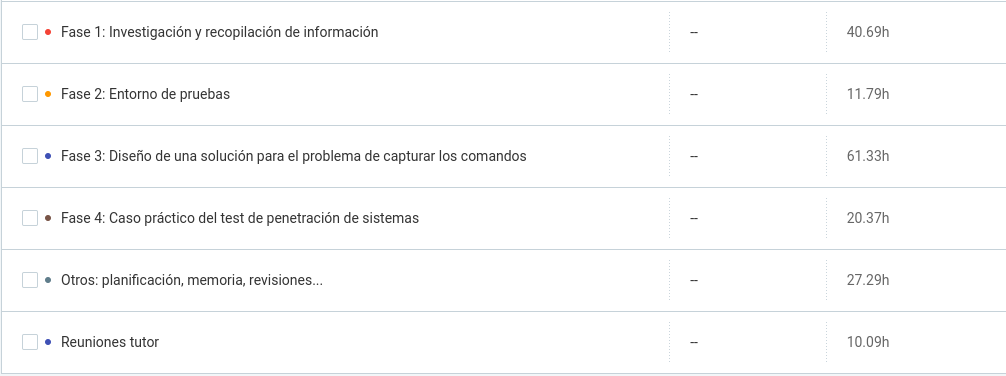
\includegraphics[width=\textwidth]{imagenes/Fases.png}
  \caption{Captura de pantalla del menú de \textbf{Clockify} dónde se aprecian las fases definidas y las horas dedicadas a cada una de ellas.}
  \label{clockifyfases}
\end{figure}


\begin{figure}[!hbt]
  \centering
  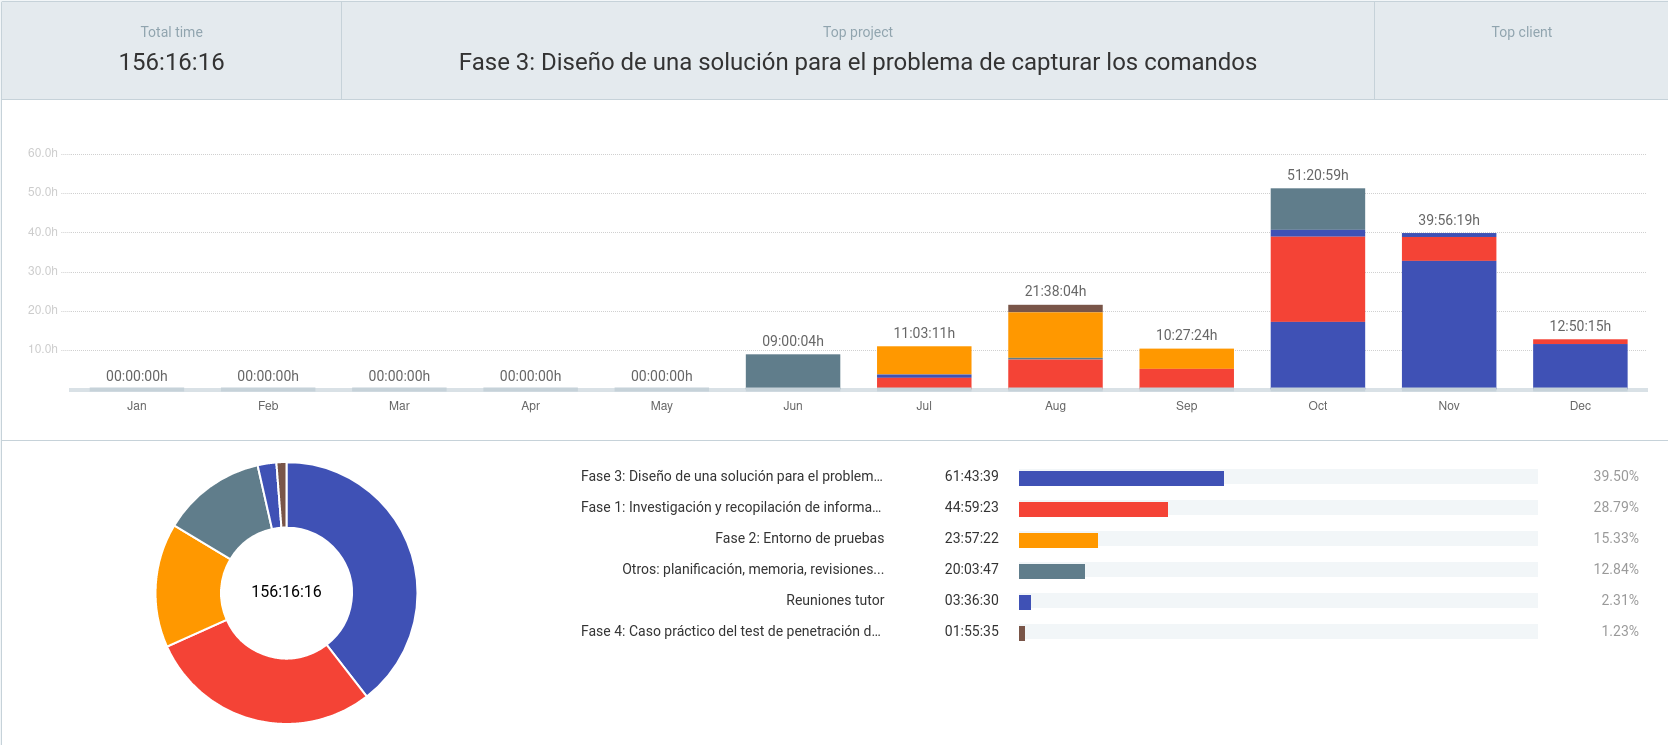
\includegraphics[width=\textwidth]{imagenes/clockifyme_1.png}
  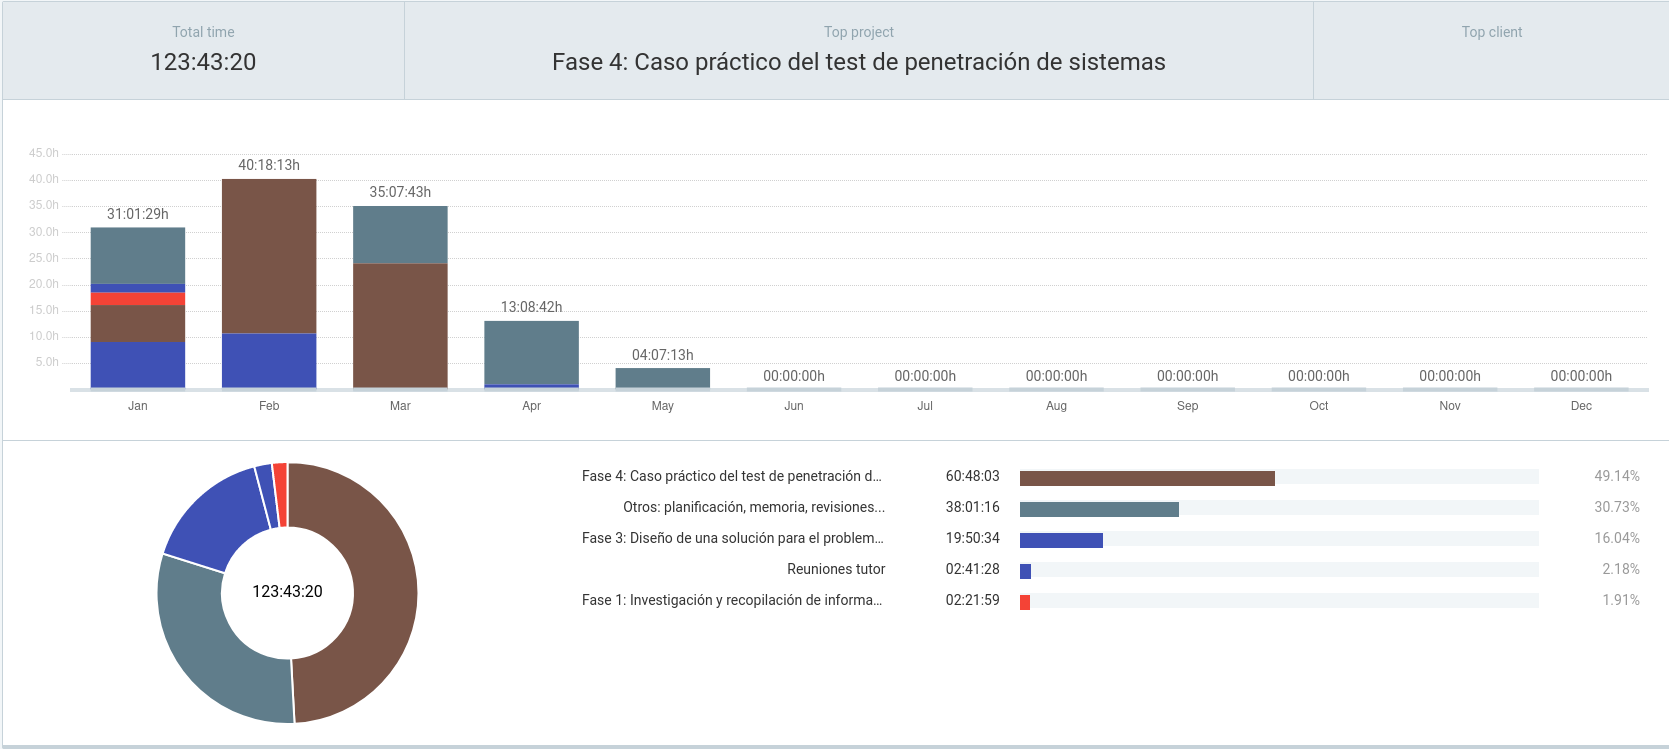
\includegraphics[width=\textwidth]{imagenes/clockifyme_2.png}
  \caption{Distribución de las horas dedicadas al proyecto por fases y por meses (durante 2020 y 2021)}
  \label{clockify_horas}
\end{figure}

\begin{figure}[!hbt]
  \centering
  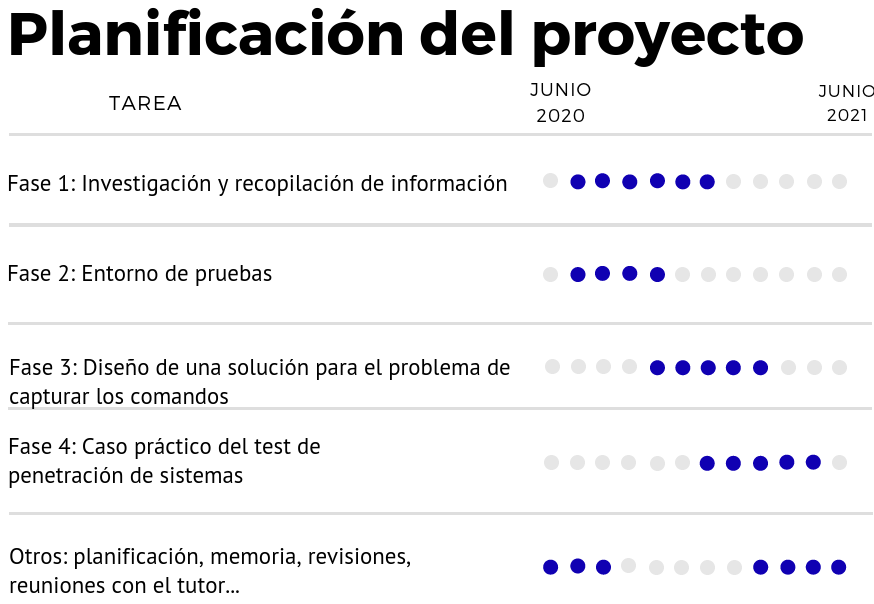
\includegraphics[width=\textwidth]{imagenes/gantt.png}
  \caption{Diagrama de Gantt con una estimación de la distribución del tiempo dedicado a cada fase de proyecto por meses (entre los meses de Junio de dos mil veinte y dos mil veintiuno. Cada punto representa un mes. Debemos tener en consideración que esta es una planificación global del proyecto, por meses y no por horas, y que la distribución de horas al mismo podría variar según el mes. Además, el hecho de que algunas fases se solapen se debe a que dependen unas de horas y es probable que haga falta dedicar tiempo de forma concurrente a varias fases a la vez. Por último, señalar que al apartado `otros' se le han marcados los meses iniciales y finales del trabajo por el esfuerzo extra que requiere la puesta en marcha del mismo y la entrega final, pero se anotará todo el tiempo dedicado a otros quehaceres fuera de las fases ya definidas y se englobará en este grupo. A la hora de crear este y otros gráficos se han tenido en cuenta las direcciones expuestas en el Capítulo 5 de  \cite{books/daglib/0076234}.}
  \label{gantt}
\end{figure}

La planificación de las horas dedicadas a cada fase se ha hecho siguiendo el diagrama de Gantt que se describe en la figura \ref{gantt}.








\section{Estimación de presupuesto}

Para finalizar la introducción del proyecto, sería interesante hacer una estimación del coste que podría haber tenido para una organización como Wazuh llevar a cabo la investigación y los desarrollos que se han dado en este proyecto. 

Se estima que se han invertido más de 300 horas (sumando la planificación, reuniones, revisiones y demás), y, dado que existe una alta posibilidad de que las personas que pudieran trabajar en una investigación como esta \textbf{no contaran con la formación previa y los conocimientos necesarios sobre hacking ético} (puesto que esto no es un requisito para trabajar como desarrollador en Wazuh), podríamos estimar que llevar a cabo un proyecto de investigación de esta índole llevaría a la empresa a dedicar a varios ingenieros, que además habrían de ser formados en la materia pertinente durante al menos unos tres meses. Además de los costes asociados a entornos de prueba en la nube y similares.

Si además se quisiera planear un desarrollo formal (más allá de la prueba de concepto que en este proyecto se plantea) que se programara en C y se integrara como parte del proyecto, el número de horas requeridas se dispararía, al igual que el número de equipos involucrados y el tiempo para llevarlo a cabo.

Por hacer una pequeña simulación, suponiendo que se emplean a tres ingenieros sin conocimientos previos sobre hacking ético y que estos deben formarse y se deben pagar algunos laboratorios para hacer pruebas, además de sus sueldos tendríamos una estimación como la de la Tabla \ref{tab:my-table}.

\begin{table}[hbt]
\begin{tabular}{|l|cccc|}
\hline
Requisito    & Cantidad & Horas/Unidad & precio/hora & Coste \\
\hline
Ingenieros   & 3      & 100             & \euro{10} & \euro{3000} \\
Formación    & 3      & 100             & \euro{1}          & \euro{300} \\
Servicios Nube & 1      & 100             & \euro{1  }         & \euro{100} \\
\hline
Total        & -      & -               & -           & \euro{3500} \\
\hline
\end{tabular}
\caption{Esta tabla plantea un posible escenario en el que una empresa empleara a tres ingenieros para realizar las labores planteadas. Dichos ingenieros tendrían que ser formados en los temas tratados (probablemente) y además requerirían algún tipo de recurso o servicios en la nube para poder realizar sus pruebas. Se ha estimado para los servicios de la nube un precio de un euro por hora basándose en los precios más bajos de recursos disponibles en Amazon Web Service \footnote{https://aws.amazon.com/es/ec2/pricing/on-demand/}.} Además, el precio de la formación se ha estimado en un euro por hora basandonos en la disponibilidad de múltiples cursos (mencionados en la sección \ref{entornos_didacticos}) que con una pequeña suscripción mensual permiten acceder a multitud de contenidos de formación en ciberseguridad, haciendo que el coste de aprendizaje por hora (de forma autónoma, sin un profesor y utilizando los recursos de la plataforma) sea más bajo.
\label{tab:my-table}
\end{table}


\bigskip
